\section{Segmentation}

\begin{frame}{Why Segmentation?}
    \begin{columns}[T]
        \begin{column}{0.55\textwidth}
            \begin{itemize}
                \item A single base-and-bounds pair requires the entire
                      address space to reside in physical memory.
                \item Large unused regions may exist between the heap
                      and the stack.
                \item \textbf{Segmentation} divides the address space into
                      logical, variable-sized segments.
                \item Typical segments: \textbf{code, heap, and stack}.
            \end{itemize}
        \end{column}

        \begin{column}{0.42\textwidth}
            \centering
            % Figure 16.1: An Address Space (Again)
            % \includegraphics[width=\textwidth]{fig16-1}
            \begin{figure}
                \centering
                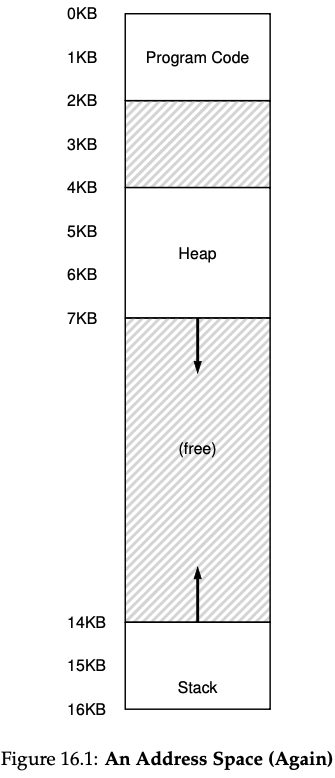
\includegraphics[width=0.6\linewidth]{figs/chapter-16/figure-16.1.png}
                \caption*{Source: chapter page 2.}
                \label{fig:figure-16.1}
            \end{figure}
        \end{column}
    \end{columns}
\end{frame}


\begin{frame}{Segmentation: Base and Bounds}
    \begin{columns}[T]
        \begin{column}{0.50\textwidth}
            \begin{itemize}
                \item Each segment has its own \textbf{base} and
                      \textbf{bounds} registers.
                \item Each segment can be independently placed in
                      physical memory.
                \item Only used portions of the address space consume
                      physical memory.
            \end{itemize}

            \medskip

            \begin{tabular}{lrr}
                \hline
                \textbf{Segment} & \textbf{Base} & \textbf{Size} \\
                \hline
                Code  & 32K & 2K \\
                Heap  & 34K & 3K \\
                Stack & 28K & 2K \\
                \hline
            \end{tabular}
        \end{column}

        \begin{column}{0.47\textwidth}
            \centering
            % Figure 16.2: Placing Segments In Physical Memory
            % \includegraphics[width=\textwidth]{fig16-2}
            \begin{figure}
                \centering
                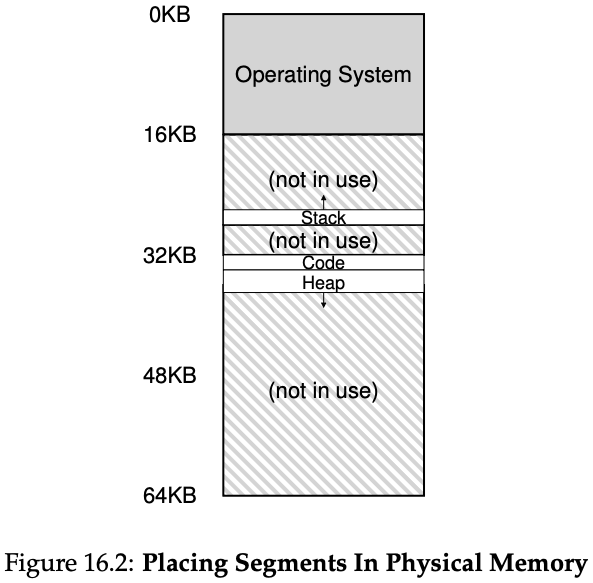
\includegraphics[width=1.1\linewidth]{figs/chapter-16/figure-16.2.png}
                \caption*{Source: chapter page 3.}
                \label{fig:figure-16.2}
            \end{figure}
        \end{column}
    \end{columns}
\end{frame}


\begin{frame}{Address Translation}
    \begin{itemize}
        \item A virtual address identifies the \textbf{segment} and
              the \textbf{offset} within it.
    \end{itemize}

    \[
        \underbrace{b_{13}b_{12}}_{\text{Segment}}
        \underbrace{b_{11}\ldots b_0}_{\text{Offset}}
    \]

    Example: virtual address $4200$:

    \[
        \underbrace{01}_{Heap}
        \underbrace{0000\,0110\,1000}_{104}
    \]

    \[
        PA = Base[Heap] + 104 = 34KB + 104 = 34920
    \]

    \begin{itemize}
        \item An out-of-bounds offset causes a
              \textbf{segmentation fault}.
    \end{itemize}
\end{frame}


\begin{frame}{What About the Stack?}
    % \begin{columns}[T]
    %     \begin{column}{0.55\textwidth}
            \begin{itemize}
                \item The stack grows toward \textbf{lower addresses}.
                \item Hardware records the growth direction of each segment.
                \item For virtual address $15$KB:
            \end{itemize}

            \[
                Offset = 3KB - 4KB = -1KB
            \]

            \[
                PA = 28KB - 1KB = 27KB
            \]
        % \end{column}
\hspace{1cm}
        % \begin{column}{0.42\textwidth}
            \centering
            % Figure 16.4:
            % Segment Registers (With Negative-Growth Support)
            % \includegraphics[width=\textwidth]{fig16-4}
            \begin{figure}
                \centering
                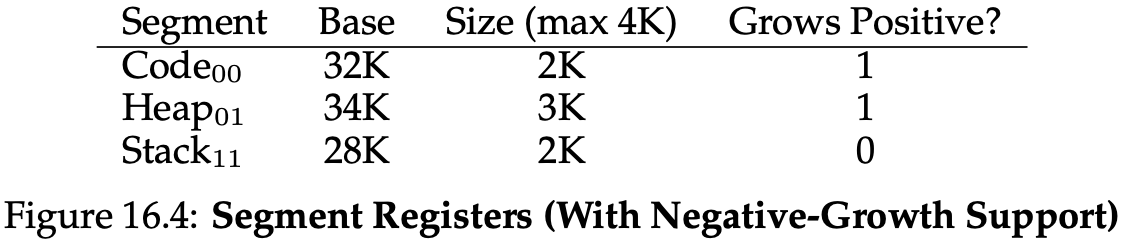
\includegraphics[width=0.8\linewidth]{figs/chapter-16/figure-16.4.png}
                \caption*{Source: chapter page 6.}
                \label{fig:figure-16.4}
            \end{figure}
    %     \end{column}
    % \end{columns}
\end{frame}


\begin{frame}{Sharing and Protection}
    % \begin{columns}[T]
    %     \begin{column}{0.53\textwidth}
            \begin{itemize}
                \item Segments can be shared among multiple address spaces.
                \item Code sharing is particularly useful.
                \item Protection bits specify whether a segment can be:
                \begin{itemize}
                    \item read,
                    \item written,
                    \item executed.
                \end{itemize}
                \item Read-only code can safely be shared by processes.
            \end{itemize}
        % \end{column}
\hspace{1cm}
        % \begin{column}{0.44\textwidth}
            \centering
            % Figure 16.5:
            % Segment Register Values (with Protection)
            % \includegraphics[width=\textwidth]{fig16-5}
            \begin{figure}
                \centering
                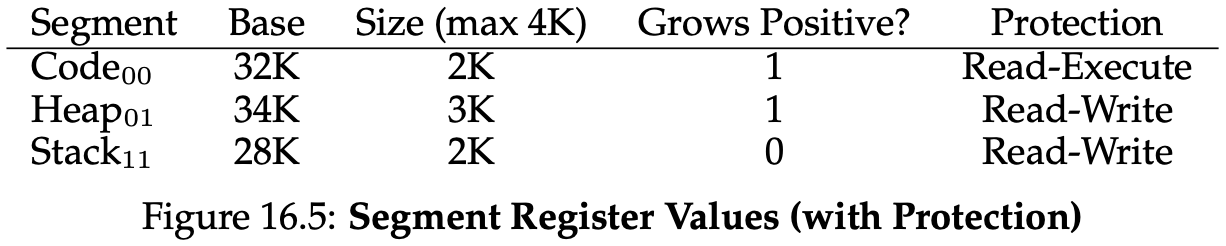
\includegraphics[width=0.8\linewidth]{figs/chapter-16/figure-16.5.png}
                \caption*{Source: chapter page 7.}
                \label{fig:placeholder}
            \end{figure}
    %     \end{column}
    % \end{columns}
\end{frame}


\begin{frame}{Coarse- vs. Fine-Grained Segmentation}
    \begin{columns}[T]
        \begin{column}{0.48\textwidth}
            \textbf{Coarse-Grained}
            \begin{itemize}
                \item Few, relatively large segments.
                \item Example: code, heap, and stack.
            \end{itemize}
        \end{column}

        \begin{column}{0.48\textwidth}
            \textbf{Fine-Grained}
            \begin{itemize}
                \item Large number of smaller segments.
                \item Requires additional hardware support.
                \item Segment tables can be stored in memory.
            \end{itemize}
        \end{column}
    \end{columns}
\end{frame}


\begin{frame}{OS Support and External Fragmentation}
    \begin{columns}[T]
        \begin{column}{0.53\textwidth}
            The OS must:
            \begin{itemize}
                \item save and restore segment registers;
                \item handle segment growth and shrinkage;
                \item manage variable-sized free regions.
            \end{itemize}

            \begin{block}{External Fragmentation}
                Free memory can become divided into small,
                non-contiguous regions, preventing large allocations.
            \end{block}
        \end{column}

        \begin{column}{0.44\textwidth}
            \centering
            % Figure 16.6:
            % Non-compacted and Compacted Memory
            % \includegraphics[width=\textwidth]{fig16-6}
            \begin{figure}
                \centering
                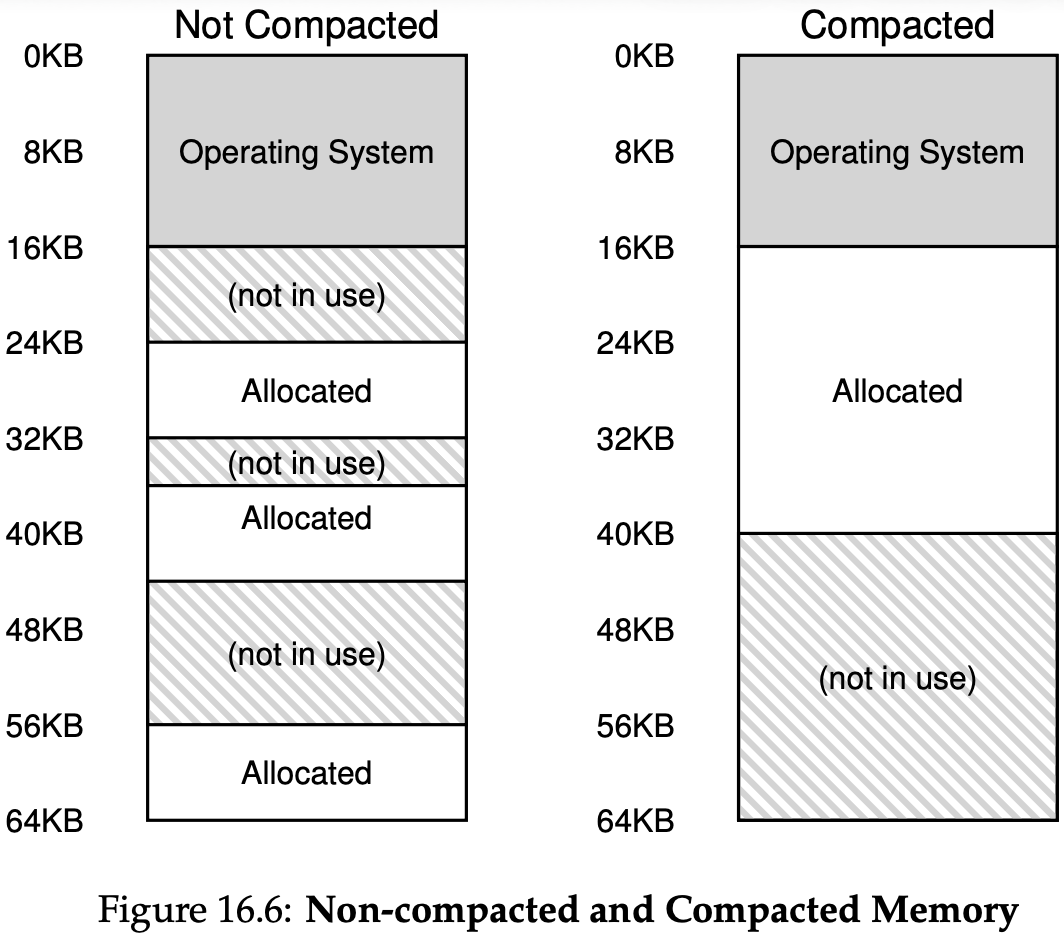
\includegraphics[width=1.1\linewidth]{figs/chapter-16/figure-16.6.png}
                \caption*{Source: chapter page 8.}
                \label{fig:figure-16.6}
            \end{figure}
        \end{column}
    \end{columns}
\end{frame}


\begin{frame}{Managing Free Space}
    \begin{itemize}
        \item \textbf{Compaction} rearranges segments to create larger
              contiguous free regions, but is expensive.
        \item Free-space allocation algorithms include:
        \begin{itemize}
            \item best-fit,
            \item worst-fit,
            \item first-fit,
            \item buddy algorithm.
        \end{itemize}
        \item External fragmentation can be minimized, but not eliminated.
    \end{itemize}
\end{frame}


\begin{frame}{Summary}
    \begin{itemize}
        \item Segmentation uses a base-and-bounds pair per logical segment.
        \item It efficiently supports large and sparse address spaces.
        \item Hardware performs relocation and bounds/protection checks.
        \item Segments can grow in different directions and can be shared.
        \item Its main limitation is \textbf{external fragmentation}.
        \item Segmentation is still not flexible enough for fully
              generalized sparse address spaces.
    \end{itemize}
\end{frame}